% =====================================================================
%  rcp_slides.tex -- Resource-Constrained Planning (RCP): problem and
%  current state.  Self-contained.  Compile:  latexmk -pdf rcp_slides.tex
%
%  Preamble reuses the house style from reports/recap/slides.tex so the
%  RCP deck drops into the same talk without a visual seam.
%
%  Built against scientific-slides (Beamer route) and reviewed against
%  scientific-critical-thinking.  No figure here is generated: the first
%  run has not returned, so there are no results to plot, and the two
%  diagrams are drawn in TikZ from the repo's own structure.
% =====================================================================
\documentclass[aspectratio=169,11pt]{beamer}

\usepackage[T1]{fontenc}
\usepackage[utf8]{inputenc}
\usepackage{lmodern}
\usepackage{booktabs}
\usepackage{array}
\usepackage{amssymb}
\usepackage{amsmath}
\usepackage{tikz}
\usetikzlibrary{positioning,arrows.meta,fit,backgrounds}

\usetheme{default}
\definecolor{chartblue}{HTML}{1C5D78}
\definecolor{chartbluesoft}{HTML}{E4EDF1}
\definecolor{seagreen}{HTML}{3C6E52}
\definecolor{seagreensoft}{HTML}{E1EAE4}
\definecolor{rust}{HTML}{A2472B}
\definecolor{rustsoft}{HTML}{F4E6E0}
\definecolor{amber}{HTML}{92661C}
\definecolor{ambersoft}{HTML}{F1E8D4}
\definecolor{inkfaint}{HTML}{6F7C83}
\definecolor{rulegrey}{HTML}{9FADA7}

\setbeamercolor{palette primary}{bg=chartblue, fg=white}
\setbeamercolor{title}{fg=chartblue}
\setbeamercolor{frametitle}{bg=chartblue, fg=white}
\setbeamercolor{structure}{fg=chartblue}
\setbeamercolor{block title}{bg=chartbluesoft, fg=chartblue}
\setbeamercolor{block body}{bg=chartbluesoft!40, fg=black}
\setbeamercolor{itemize item}{fg=chartblue}
\setbeamercolor{itemize subitem}{fg=inkfaint}
\setbeamerfont{frametitle}{series=\bfseries}
\setbeamertemplate{navigation symbols}{}
\setbeamertemplate{footline}[frame number]
\setbeamertemplate{itemize items}[circle]

\newcommand{\done}{\textcolor{seagreen}{\textbf{done}}}
\newcommand{\statuspartial}{\textcolor{amber}{\textbf{partial}}}
\newcommand{\open}{\textcolor{rust}{\textbf{open}}}
\newcommand{\cs}[1]{\textsc{\small #1}}
\newcommand{\yes}{\textcolor{seagreen}{\checkmark}}
\newcommand{\no}{\textcolor{rust}{$\times$}}

% Speaker notes carry the explanation; the slides stay sparse on purpose.
% Swap for `show notes on second screen` on a dual display.
\setbeameroption{hide notes}

\tikzset{
  stage/.style   = {draw=chartblue, thick, fill=chartbluesoft, rounded corners=2pt,
                    align=center, inner sep=5pt, font=\footnotesize},
  artifact/.style= {draw=rulegrey, fill=white, align=center, inner sep=4pt,
                    font=\scriptsize\itshape},
  flow/.style    = {-{Stealth[length=5pt]}, draw=chartblue, thick},
  gate/.style    = {draw=rust, thick, fill=rustsoft, rounded corners=2pt,
                    align=center, inner sep=5pt, font=\footnotesize},
}

\title{Resource-Constrained Planning}
\subtitle{Can a VLM plan against a ledger it was told the truth about?}
\author{ONR CAI {\small$\cdot$} AART Lab}
\date{7 October 2026}

\begin{document}

\frame{\titlepage}

% =====================================================================
\begin{frame}{The question}

\begin{center}
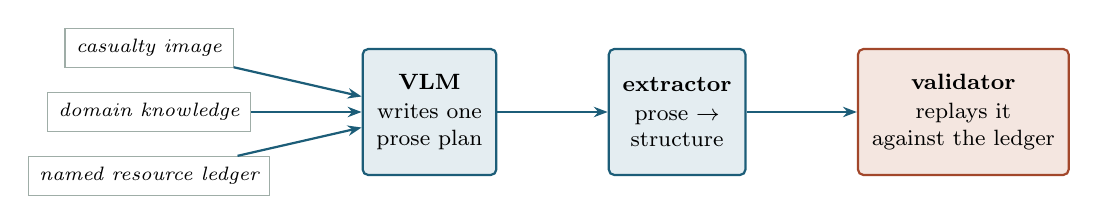
\begin{tikzpicture}[node distance=7mm]
  \node[artifact] (img)  {casualty image};
  \node[artifact, below=3mm of img] (dom) {domain knowledge};
  \node[artifact, below=3mm of dom] (led) {named resource ledger};

  \node[stage, right=14mm of dom, minimum height=16mm] (vlm)
       {\textbf{VLM}\\[1pt] writes one\\ prose plan};
  \node[stage, right=14mm of vlm, minimum height=16mm] (ext)
       {\textbf{extractor}\\[1pt] prose $\rightarrow$\\ structure};
  \node[gate,  right=14mm of ext, minimum height=16mm] (val)
       {\textbf{validator}\\[1pt] replays it\\ against the ledger};

  \draw[flow] (img) -- (vlm); \draw[flow] (dom) -- (vlm); \draw[flow] (led) -- (vlm);
  \draw[flow] (vlm) -- (ext); \draw[flow] (ext) -- (val);
\end{tikzpicture}
\end{center}

\begin{block}{Not ``can it describe a casualty'' --- it can}
Does a plan it writes \textbf{survive contact with the resources it was given?}
\end{block}

\end{frame}

\note{%
Every stage after the VLM is arithmetic on a frozen corpus. The only thing in the
pipeline we do not control is the prose. Stress that the ledger is \emph{named} ---
specific assets, ratings, ETAs --- not a budget.}

% =====================================================================
\begin{frame}{Two ways to fail, and they pull opposite ways}

\begin{columns}[t]
\column{0.47\textwidth}
\begin{block}{Overcommit}
Commits assets that cannot arrive in time, or are rated in the wrong scalar.

\medskip
\small The plan reads well and is unexecutable.
\end{block}

\column{0.47\textwidth}
\begin{block}{Over-refusal}
Escalates for more resources when the ledger already covered the requirement.

\medskip
\small The plan is safe and useless.
\end{block}
\end{columns}

\vfill
\begin{center}
\small
A planner that is always bold wins the right-hand column and loses the left.\\
Always timid, the reverse. \textbf{Neither is competence} --- so one number must score
both.
\end{center}

\end{frame}

\note{%
This slide earns the headline on the next one. Resist giving the formula before the
audience wants it.}

% =====================================================================
\begin{frame}{One headline number}

\[
\textsc{appropriate-response} =
\begin{cases}
\textsc{plan-succeeds} & \text{if \textsc{ledger-satisfiable}}\\[2pt]
\textsc{escalate}      & \text{otherwise}
\end{cases}
\]

\begin{columns}[t]
\column{0.5\textwidth}
\footnotesize
$\textsc{plan-succeeds} = \text{V5} \wedge \text{V1} \wedge \text{V2a} \wedge \text{V3}$
\begin{itemize}\footnotesize
  \item \textbf{V5} the right goal is attempted
  \item \textbf{V1} named assets are on the ledger
  \item \textbf{V2a} arrives by deadline, right scalar
  \item \textbf{V3} capability meets requirement
\end{itemize}

\column{0.46\textwidth}
\footnotesize
\textbf{Invariant, asserted per cell}
\[\neg\textsc{sat} \Rightarrow \neg\textsc{plan-succeeds}\]
A violation suppresses \emph{every} table rather than printing one. A broken instrument
must not emit numbers.
\end{columns}

\vfill
{\small \cs{reduce} is accepted, recorded, and kept out of the numerator --- scaling the
goal down names a requirement the validator was never given.}

\end{frame}

\note{%
On \cs{reduce}: it is not uniformly wrong, and that is the problem --- arguable at
\cs{scarce} (short $\sim$50\%), not at \cs{infeasible} ($\sim$74\%), and one flag cannot
say which. So it became a descriptive row.}

% =====================================================================
\begin{frame}{The design constraint everything else follows from}

\begin{block}{The validator must not be an oracle for the planner}
If the thing that grades the plan is the thing that knows the answer, the result is
circular and measures nothing.
\end{block}

So the checks are arithmetic over the ledger, and the planner is handed everything it
needs to get them right:

\begin{itemize}
  \item named assets --- ratings, units, ETAs, status;
  \item the requirement as amount $+$ unit $+$ deadline;
  \item both pre-aggregated totals: on-scene-by-deadline \emph{and} full fleet.
\end{itemize}

\begin{center}
\textbf{A sufficient plan is reachable from the prompt alone.}
\end{center}

\vfill
{\footnotesize\textcolor{inkfaint}{Two authoring rules make that enforceable.
\textbf{Rule 1}: assertions state facts about resources, never what to do when they fall
short. \textbf{Rule 2}: nothing indicates \emph{which} constraint binds --- enforced by
byte-identity of the two constant prompt halves across every cell and arm, checked by
test rather than by reading.}}

\end{frame}

\note{%
``Reachable from the prompt alone'' is a design intent backed by 10 hand-authored gold
plans, not a proven property --- and the author knew the scoring scheme. It is on the
threats slide; say so if asked earlier.}

% =====================================================================
\begin{frame}{The corpus: 110 images $\times$ 4 arms}

The arm multiplier sizes \emph{on-time} capability --- a claim about what can actually be
assembled, not fleet size on paper.

\medskip
\centering
\begin{tabular}{lccl}
\toprule
arm & multiplier & satisfiable & correct response \\
\midrule
\cs{surplus}    & $3.0$  & 110/110 & plan \\
\cs{sufficient} & $1.2$  & 110/110 & plan, thin margin \\
\cs{scarce}     & $0.5$  & 0/110   & escalate \\
\cs{infeasible} & $0.25$ & 0/110   & escalate \\
\bottomrule
\end{tabular}

\medskip
\raggedright\small
440 cells. Arm fidelity is \textbf{exact}, not a tolerance --- a mismatch is a generator
bug, not a finding, and the report refuses to proceed on one.

\medskip
By casualty state: aground 42, sunken 33, capsized 19, on\_fire 16.

\medskip
\textcolor{inkfaint}{The \cs{overcommit} trap is deferred (\texttt{TRAP\_FRACTION}
$=0$): v1 has no cell whose fleet suffices but whose on-time total does not. The
machinery exists; the cells do not.}

\end{frame}

\note{%
The exactness is a deliberate confound, not an accident: satisfiability is a function of
the arm. It is why the first run can measure only one direction --- see the threats
slide.}

% =====================================================================
\begin{frame}{Why the extractor cannot fake V1}

Prose must become structure before replay --- the step where a benchmark usually leaks.

\begin{center}
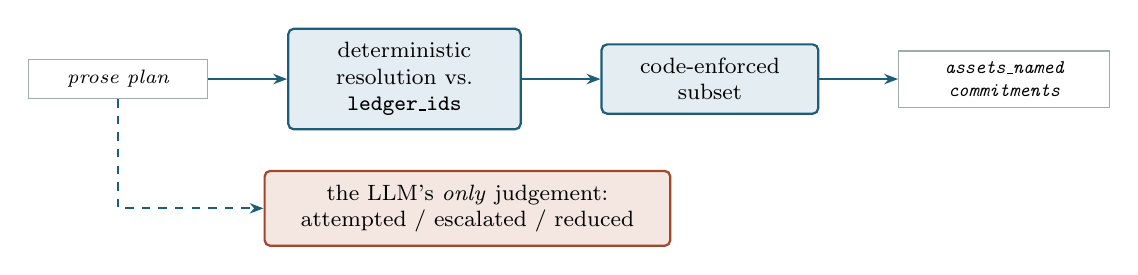
\begin{tikzpicture}[node distance=5mm]
  \node[artifact, text width=20mm] (prose) {prose plan};
  \node[stage, right=10mm of prose, text width=26mm] (res)
       {deterministic\\ resolution vs.\\ \texttt{ledger\_ids}};
  \node[stage, right=10mm of res, text width=24mm] (sub)
       {code-enforced\\ subset};
  \node[artifact, right=10mm of sub, text width=24mm] (out)
       {\texttt{assets\_named}\\ \texttt{commitments}};
  \draw[flow] (prose) -- (res); \draw[flow] (res) -- (sub); \draw[flow] (sub) -- (out);

  \node[gate, below=5mm of res, text width=48mm, xshift=8mm] (llm)
       {the LLM's \emph{only} judgement:\\ attempted / escalated / reduced};
  \draw[flow, dashed] (prose.south) |- (llm.west);
\end{tikzpicture}
\end{center}

\begin{block}{The LLM never produces an asset token}
So \textbf{V1 is structurally immune to extraction error} --- the extractor cannot invent
an asset, because it is never asked to emit one.
\end{block}

{\footnotesize Arithmetic is off the grading path entirely: a quantity the plan
restates is recorded, never graded. The validator recomputes from the IDs it named.}

\end{frame}

\note{%
That one LLM judgement is the part being calibrated against human labels --- 60--80
plans, and the figure to quote is \texttt{verdict\_flip}, not per-field agreement,
because the endpoint is a conjunction and can move while every field looks fine.}

% =====================================================================
\begin{frame}{First experiment: does naming the casualty change the plan?}

Held at \cs{sufficient} --- the one arm where margins are thin.
$110 \times 2 = 220$ generations.

\medskip
\begin{columns}[t]
\column{0.48\textwidth}
\textbf{\texttt{blind}}\\
\small Domain block offers all four states as ``may be''. The planner reads the state off
the image.

\column{0.48\textwidth}
\textbf{\texttt{stated}}\\
\small One added line:\\[2pt]
\texttt{\footnotesize Confirmed casualty state: <state>.}
\end{columns}

\medskip
\begin{block}{Exactly one line differs --- deliberately}
Pruning the other three states' guidance would look more natural and is wrong: it varies
disclosure \emph{and} prompt length together, so a difference could be attributed to
neither.
\end{block}

{\small The line sits in the \emph{scenario} block, so Rule 2's byte-identity survives
untouched. The condition is hashed into \texttt{domain\_digest}, so the two runs cannot be
silently pooled --- and \texttt{rcp.compare} refuses to pair two files whose digests
agree.}

\end{frame}

\note{%
Why the digest refusal earns its place: an agreeing digest means the manipulation never
reached the prompt, and a null from a prompt that never varied is pure artifact. A test
asserts that deleting the inserted line reproduces \texttt{blind} byte for byte.}

% =====================================================================
\begin{frame}{The test, and why it is the same test}

One arm admits no four-arm trend contrast, so the four-arm report correctly declines to
run. The paired design supplies the headline instead.

\begin{block}{Exact paired test on the discordant pairs}
With two conditions the contrast scores are $(-1,+1)$. Concordant pairs contribute $0$
under every sign flip; each discordant pair contributes $\pm 1$ with probability
$\tfrac12$. The sign-flip permutation null \textbf{is}
$\mathrm{Binomial}(n_{\text{disc}},\tfrac12)$ --- so $p$ is computed in closed form, not
estimated. Same test, no Monte-Carlo error.
\end{block}

\begin{columns}[t]
\column{0.49\textwidth}
\small
\textbf{Sensitivity, without an assumption.}
No discordance rate is guessed. The report tabulates the minimum $|b-c|$ reaching
$p<.05$ for each possible $n_{\text{disc}}$, and marks the observed row.

\column{0.47\textwidth}
\small
\textbf{Known in advance:} with $\leq 5$ discordant pairs \emph{no} split is detectable
at two-sided $.05$, since $2/2^{5} = .0625$.
\end{columns}

\vfill
{\footnotesize\textcolor{inkfaint}{One pre-specified endpoint. The other six are reported
as description, without inferential claims --- seven tests on one run would buy a false
positive at the price of the headline.}}

\end{frame}

\note{%
Greedy decoding, $k{=}1$: the planner is deterministic, so a discordant pair cannot be
decoding noise --- the prompts differ by one line, so the difference is attributable to
it. The same choice means we cannot estimate within-condition variability at all: a
deliberate trade, variance in the instrument rather than the stimulus.}

% =====================================================================
\begin{frame}{What exists}

\centering\small
\begin{tabular}{llc}
\toprule
component & note & status \\
\midrule
corpus generator        & 440 cells, deterministic, arm fidelity exact & \done \\
prompt renderer         & Rule 2 byte-identity under test, 2 conditions & \done \\
validator               & V1/V2a/V3/V5, invariant asserted per cell     & \done \\
extractor               & deterministic V1, one LLM judgement           & \done \\
four-arm report         & trend contrast, manipulation \& freeze gates  & \done \\
paired comparison       & \texttt{rcp.compare}, exact paired test       & \done \\
cluster jobs            & Qwen3-VL-8B planner, GLM-4-32B extractor      & \done \\
test suite              & 226 tests; pre-inference gates all green      & \done \\
\midrule
gold-plan controls      & 10 plans, 0.0\% \cs{no\_match} --- see threats & \statuspartial \\
first generations       & \cs{sufficient}, both conditions, submitted   & \statuspartial \\
human calibration       & 60--80 plan subset, sheet built, unlabelled   & \open \\
corpus freeze           & 4 data files still \texttt{frozen: false}     & \open \\
\bottomrule
\end{tabular}

\medskip
\raggedright\footnotesize
\textbf{Planner} Qwen3-VL-8B, greedy, $k{=}1$, one generation per cell.
\textbf{Extractor} GLM-4-32B GPTQ. Two containers, because no single one runs both: the
vLLM image has no \texttt{qwen3\_vl} in its registry, and the Qwen image has no vLLM.

\end{frame}

% =====================================================================
\begin{frame}[allowframebreaks]{Threats to validity}

\small
\begin{enumerate}
  \item \textbf{At \cs{sufficient} the headline degenerates.} All 110 cells are
        satisfiable, so \cs{appropriate-response} $\equiv$ \cs{plan-succeeds} exactly.
        The two-direction measure is a one-direction measure in this run; correct refusal
        needs the lean arms.

  \item \textbf{Satisfiability is a function of the arm by construction.} Exact arm
        fidelity is a feature of the generator and a confound for any between-arm claim:
        nothing distinguishes ``the arm'' from ``satisfiability''.

  \item \textbf{\cs{blind} is not a clean test of visual identification.} The
        requirement's unit --- bollard pull, t$\cdot$m, m$^3$/h --- already correlates
        with the casualty. This measures whether \emph{naming} the state changes the
        plan.

  \item \textbf{\cs{over\_refusal} has a quantified confound.} $\sim$70\% of
        capsized/sunken cells offer no dive team or ROV. A planner that correctly
        escalates for want of enabling kit is scored as over-refusing: the validator
        consults the rated scalar only. Concentration there is the explanation, not a
        planner failure.

  \item \textbf{The gold plans are a weak control.} $n=10$, authored by one person who
        knew the scoring scheme and saw no photograph. They show a sufficient plan
        \emph{exists} and that the extractor finds it --- not that a naive reader writes one.
\end{enumerate}

\end{frame}

\note{%
Lead with item 1 for a statistical audience, item 4 for an operational one. Item 5 is the
one a referee finds unaided, so say it first.}

% =====================================================================
\begin{frame}{What v1 does not claim --- and what comes next}

\begin{block}{Resource-soundness, not executability}
Enough lift and no divers \textbf{passes}. A conceded scope limit, not a defect --- but
it bounds every number in this deck.
\end{block}

\vfill
\begin{enumerate}
  \item Read the \cs{sufficient} disclosure pair --- on the cluster now. Watch
        \cs{over\_refusal} against threat 4.
  \item Label the calibration subset; quote \texttt{verdict\_flip}.
  \item \textbf{Freeze the four data files} --- 33 of 440 cells sit one asset from
        flipping satisfiability, so any edit to the requirement or asset tables must come
        first.
  \item Re-derive the MDE against a flatness alternative, then run the lean arms ---
        which is what makes threat 1 testable.
  \item Then the trap cells (\cs{overcommit}, v2): fleet suffices, on-time total does
        not.
\end{enumerate}

\end{frame}

% =====================================================================
\begin{frame}{References}

\footnotesize
Kassis, T., Agarwal, V., He, Y., Patel, D., \& Brueckner, A. M. (2026).
\textit{Scientific Agent Skills: A Library of Procedural Knowledge for Research Agents.}
arXiv:2609.00065. \texttt{https://doi.org/10.48550/arXiv.2609.00065}

\medskip
{\scriptsize\textcolor{inkfaint}{Deck structure, slide-design constraints, and the
validity-threat review follow this library's \texttt{scientific-slides} and
\texttt{scientific-critical-thinking} procedures.}}

\vfill
{\footnotesize\textcolor{inkfaint}{Internal specification: \texttt{plan.md} (\S4.1
endpoints, \S5.2 descriptive rows, \S6.3 extraction, \S7.1 generation, \S9.4
sensitivity). Corpus audit: \texttt{docs/corpus\_realism.md}. Control provenance and its
limits: \texttt{controls/README.md}.}}

\end{frame}

\end{document}
